% !TeX spellcheck = pl_PL
% Options for packages loaded elsewhere
\PassOptionsToPackage{unicode}{hyperref}
\PassOptionsToPackage{hyphens}{url}
%
\documentclass[a4paper,12pt
]{article}
\usepackage{times,fullpage,polski}
\usepackage{amssymb,amsmath}
\usepackage{ifxetex,ifluatex}
\ifnum 0\ifxetex 1\fi\ifluatex 1\fi=0 % if pdftex
  \usepackage[T1]{fontenc}
  \usepackage[utf8]{inputenc}
  \usepackage{textcomp} % provide euro and other symbols
\else % if luatex or xetex
  \usepackage{unicode-math}
  \defaultfontfeatures{Scale=MatchLowercase}
  \defaultfontfeatures[\rmfamily]{Ligatures=TeX,Scale=1}
\fi
% Use upquote if available, for straight quotes in verbatim environments
\IfFileExists{upquote.sty}{\usepackage{upquote}}{}
\IfFileExists{microtype.sty}{% use microtype if available
  \usepackage[]{microtype}
  \UseMicrotypeSet[protrusion]{basicmath} % disable protrusion for tt fonts
}{}
\makeatletter
\@ifundefined{KOMAClassName}{% if non-KOMA class
  \IfFileExists{parskip.sty}{%
    \usepackage{parskip}
  }{% else
    \setlength{\parindent}{0pt}
    \setlength{\parskip}{6pt plus 2pt minus 1pt}}
}{% if KOMA class
  \KOMAoptions{parskip=half}}
\makeatother
\usepackage{xcolor}
\IfFileExists{xurl.sty}{\usepackage{xurl}}{} % add URL line breaks if available
\IfFileExists{bookmark.sty}{\usepackage{bookmark}}{\usepackage{hyperref}}
\hypersetup{
  hidelinks,
  pdfcreator={LaTeX via pandoc}}
\urlstyle{same} % disable monospaced font for URLs
\usepackage{graphicx}
\makeatletter
\def\maxwidth{\ifdim\Gin@nat@width>\linewidth\linewidth\else\Gin@nat@width\fi}
\def\maxheight{\ifdim\Gin@nat@height>\textheight\textheight\else\Gin@nat@height\fi}
\makeatother
% Scale images if necessary, so that they will not overflow the page
% margins by default, and it is still possible to overwrite the defaults
% using explicit options in \includegraphics[width, height, ...]{}
\setkeys{Gin}{width=\maxwidth,height=\maxheight,keepaspectratio}
% Set default figure placement to htbp
\makeatletter
\def\fps@figure{htbp}
\makeatother
\setlength{\emergencystretch}{3em} % prevent overfull lines
\providecommand{\tightlist}{%
  \setlength{\itemsep}{0pt}\setlength{\parskip}{0pt}}
\setcounter{secnumdepth}{-\maxdimen} % remove section numbering

\usepackage{listings}
\lstset{language=Python}

\begin{document}


\title{Rozwiązania chmurowe dla obliczeń
kwantowych\\ {\normalsize Stan na październik
2022}}

\author{Jarosław Miszczak}
\date{26/04/2023}

\maketitle

\begin{abstract}
Raport przedstawia przegląd systemów programowania komputerów kwantowych
dedykowanych dla sprzętu bazującego na obliczeniach optycznych oraz na
automach neutalnych. Zaprezentowane są rozwiązanie dwóch firm
produkujących tego typu urządzenia oraz oferujących dostęp do
oprogramowanie dedykowanego do obsługi dedykowanych systemów.
Przedstawiony p0rzegląd jest uzupełnieniem dla przeglądu przygotowanego na potrzeby projektu w październiku 2022.
\end{abstract}


\hypertarget{platforma-pulser-studio-firmy-pasqal}{%
\section{Platforma Pulser Studio firmy
Pasqal}\label{platforma-pulser-studio-firmy-pasqal}}

\hypertarget{podstawowe-cechy}{%
\subsection{Podstawowe cechy}\label{podstawowe-cechy}}

Pulser Studio to platforma firmy Pasqal, która umożliwia użytkownikom
projektowanie, symulowanie i uruchamianie algorytmów kwantowych na
urządzeniach kwantowych tworzonych przez tą firmę. Platforma Pulser
Studio pozwala na tworzenie programów kwantowych przy użyciu języka
programowania Python, który jest jednym z najpopularniejszych języków
programowania w dziedzinie kwantowych obliczeń. Pulser Studio umożliwia
tworzenie sekwencji impulsów, które są potrzebne do wykonania obliczeń
kwantowych na urządzeniach kwantowych firmy Pasqal.

\begin{figure}
\centering
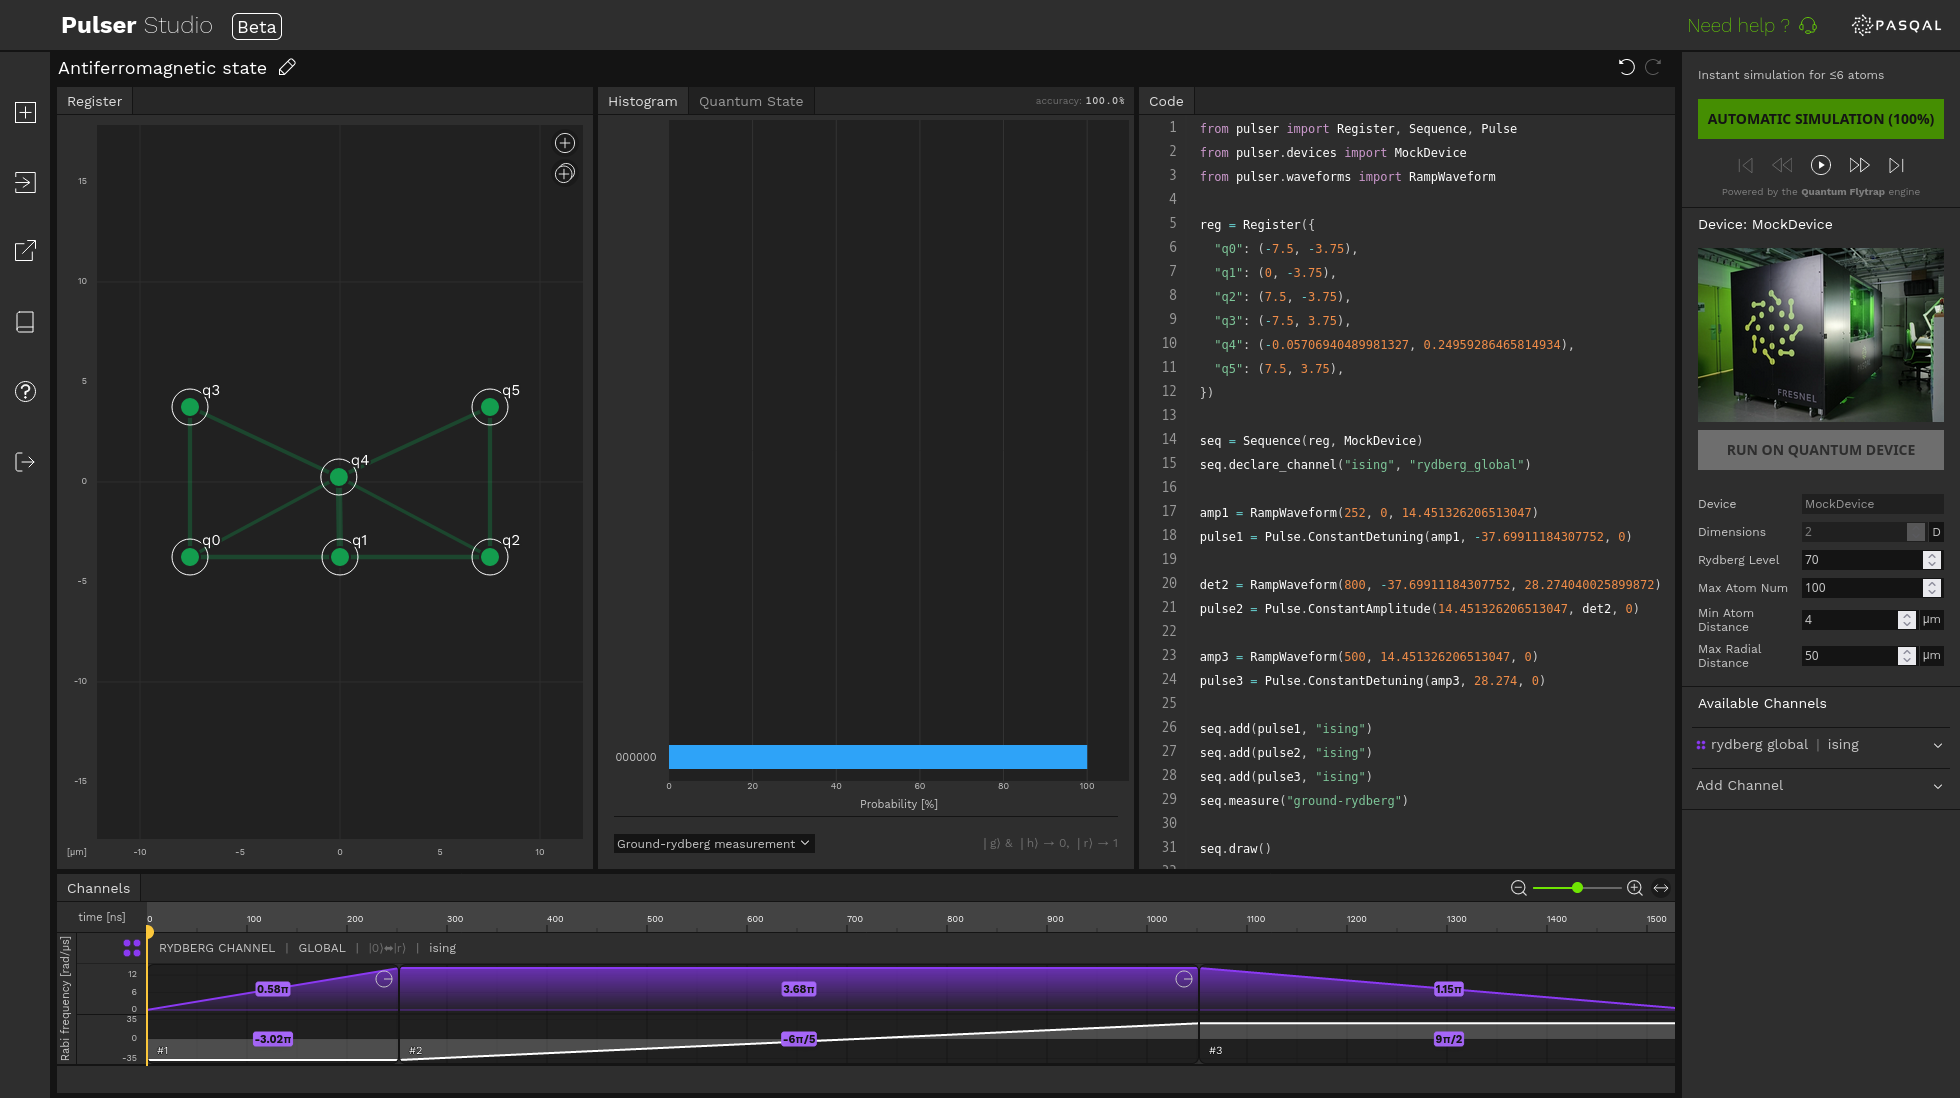
\includegraphics{Pulser-Studio-basic-view.png}
\caption{Widok interfejsu użytkownika platformy Pulsar Studio. Interfejs pozwala na konfigurację topologi połączeń oraz kontrolę nad siłą połączeń. Dodatkowo generowany jest kod źródłowy w języku Python}
\end{figure}

Pulser Studio zapewnia narzędzia do symulacji obliczeń kwantowych na
komputerze klasycznym przed ich uruchomieniem na urządzeniu kwantowym.
Rozszerzenie \texttt{pulser\_simulation} dostarcza narzędzi do
klasycznej symulacji (z wykorzystaniem bibliotek QuTiP), aby wspomóc
rozwój i testowanie nowych sekwencji impulsów. To umożliwia użytkownikom
testowanie i optymalizowanie swoich algorytmów przed ich implementacją
na rzeczywistych urządzeniach kwantowych.

\hypertarget{zasada-dziaux142ania}{%
\subsection{Zasada działania}\label{zasada-dziaux142ania}}

Pulser został zaprojektowany tak, aby umożliwić użytkownikom tworzenie
eksperymentów dostosowanych do konkretnych urządzeń z neutralnym atomem.
Zmniejsza to poziom abstrakcji i daje maksymalną elastyczność i kontrolę
nad zachowaniem odpowiednich parametrów fizycznych, w granicach
wyznaczonych przez wybrane urządzenie.

W konsekwencji oprogramowaie Pulser wyłamuje się z paradygmatu cyfrowych
obliczeń kwantowych i umożliwia również tworzenie analogowych symulacji
kwantowych, które wykraczają poza tradycyjne podejście do tworzenia
obwodów kwantowych. Niezależnie od rodzaju eksperymentu lub paradygmatu,
jeśli można go wykonać na urządzeniu, można go wykonać za pomocą
Pulsera.

\begin{figure}
\centering
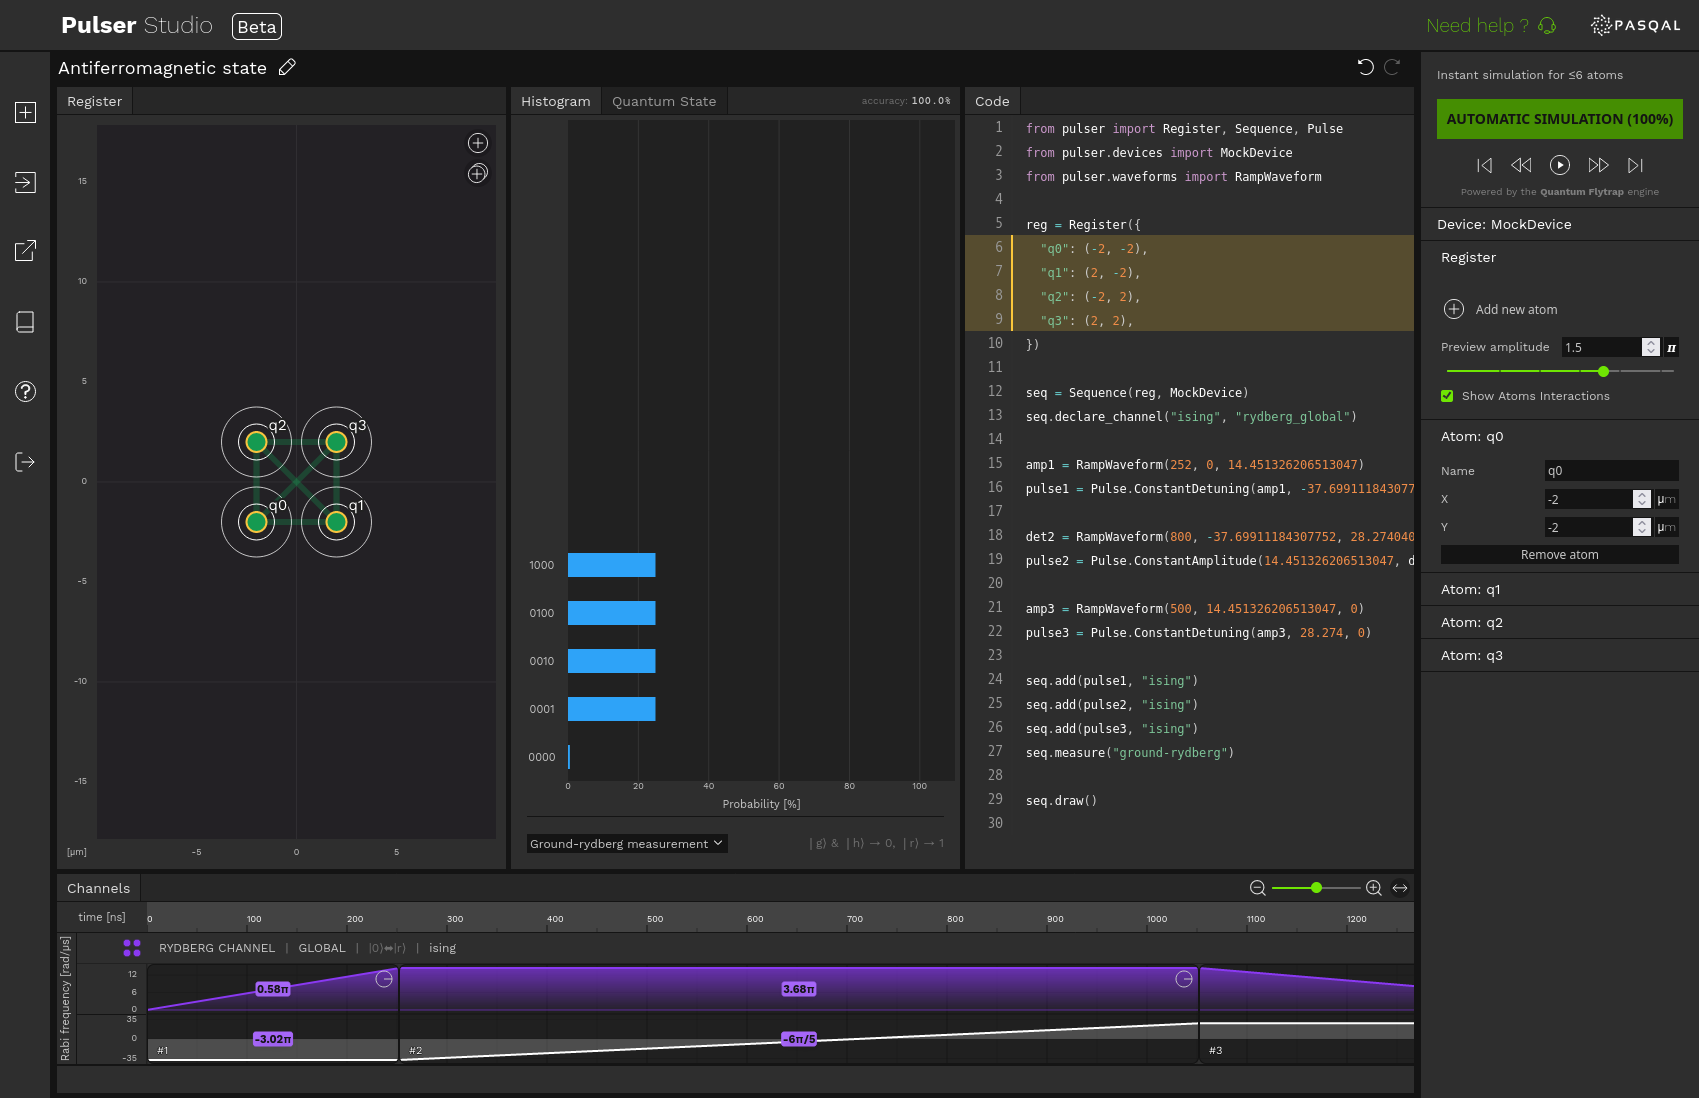
\includegraphics{Pulser-Studio-simulation-results-001.png}
\caption{Wynik symulacji wykonanej za pomocą platformy Pulsar Studio. }
\end{figure}

\begin{lstlisting}
from pulser import Register, Sequence, Pulse
from pulser.devices import MockDevice
from pulser.waveforms import RampWaveform

reg = Register({
  "q0": (-2, -2),
  "q1": (2, -2),
  "q2": (-2, 2),
  "q3": (2, 2),
})

seq = Sequence(reg, MockDevice)
seq.declare_channel("ising", "rydberg_global")

amp1 = RampWaveform(252, 0, 14.451326206513047)
pulse1 = Pulse.ConstantDetuning(amp1, -37.69911184307752, 0)

det2 = RampWaveform(800, -37.69911184307752, 28.274040025899872)
pulse2 = Pulse.ConstantAmplitude(14.451326206513047, det2, 0)

amp3 = RampWaveform(500, 14.451326206513047, 0)
pulse3 = Pulse.ConstantDetuning(amp3, 28.274, 0)

seq.add(pulse1, "ising")
seq.add(pulse2, "ising")
seq.add(pulse3, "ising")
seq.measure("ground-rydberg")

seq.draw()
\end{lstlisting}


Dodatkowo platforma Pulser Studio udostępnia narzędzia do monitorowania
i debugowania stanu pracy urządzenia kwantowego w czasie rzeczywistym.
Umożliwia to użytkownikom lepszą kontrolę nad zadaniami obliczeniowymi
przesłanymi do komputera kwantowego.

Pulser Studio jest zintegrowany z chmurą kwantową firmy Pasqal, co
umożliwia użytkownikom dostęp do wysokiej jakości urządzeń kwantowych i
zapewnia wysoką skalowalność.

\hypertarget{platforma-firmy-quandela}{%
\section{Platforma firmy
Quandela}\label{platforma-firmy-quandela}}

Komputery kwantowe firmy Quandela opierają się na manipulacji światłem
za pomocą układów fotonicznych.

\hypertarget{quandela-cloud}{%
\paragraph{Quandela Cloud}\label{quandela-cloud}}

\begin{figure}
\centering
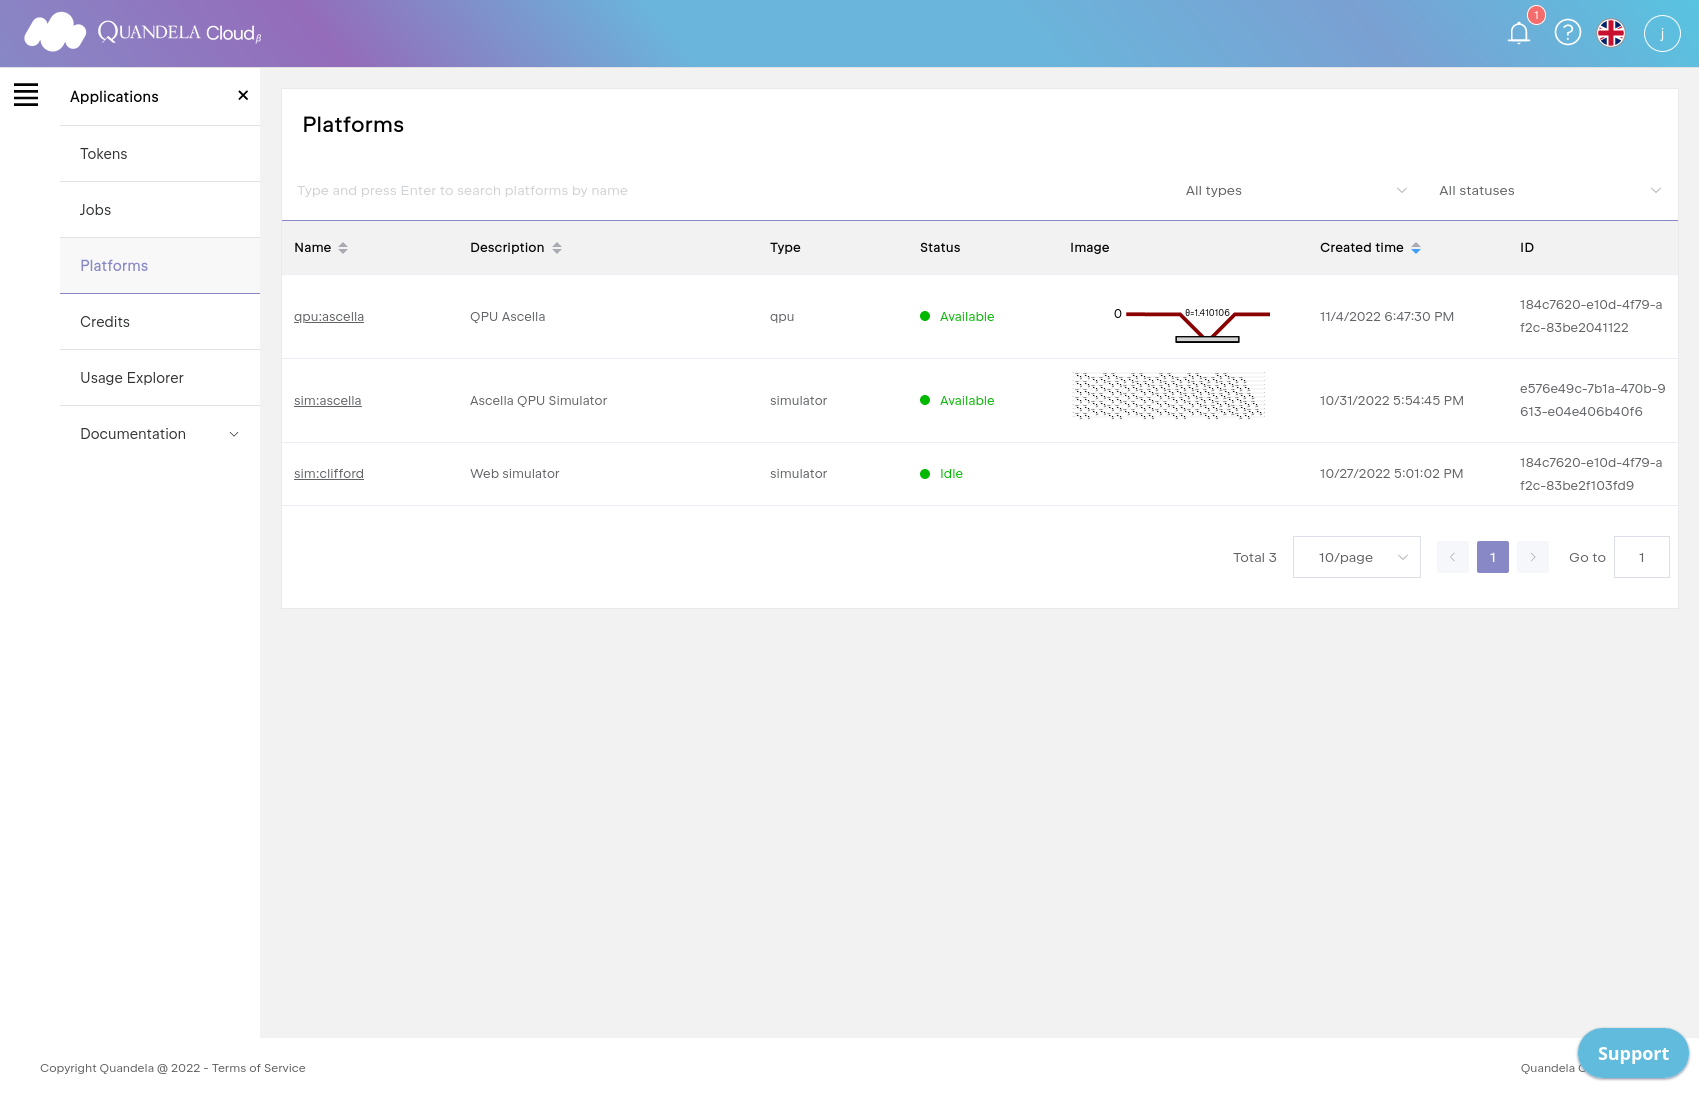
\includegraphics{Quandela-IDE-Platforms.png}
\caption{Informacja o platfromach dostępnych z poziomu Quandela Cloud}
\end{figure}

\hypertarget{parceval}{%
\subsection{Parceval}\label{parceval}}

Parceval to oprogramowanie opracowane przez firmę Quandela do
programowania i sterowania kwantowymi komputerami fotonicznymi.
Parceval został stworzony w celu ułatwienia procesu programowania i
obsługi tych złożonych systemów, aby umożliwić użytkownikom skupienie
się na projektowaniu i przeprowadzaniu eksperymentów na komputerach
fotonicznych.

Oprogramowanie Parseval umożliwia użytkownikom tworzenie programów
obliczeniowych za pomocą języków programowania, takich jak Python i C++,
które następnie mogą być przesłane do komputera kwantowego lub
fotonicznego firmy Quandela. Parseval umożliwia również użytkownikom
tworzenie schematów logicznych i grafów obliczeniowych, które mogą być
wykorzystane do przeprowadzania obliczeń na komputerze kwantowym lub
fotonicznym.

Parseval jest również wyposażony w funkcje do debugowania i testowania
kodu, co umożliwia użytkownikom szybkie iterowanie i poprawianie kodu.
Parseval oferuje również narzędzia do wizualizacji danych i wyników
obliczeń, co umożliwia użytkownikom analizę i interpretację wyników.

\begin{lstlisting}
import perceval as pcvl
import sympy as sp
import numpy as np

cnot = pcvl.Circuit(6, name="Ralph CNOT")
cnot.add((0, 1), pcvl.BS.H(pcvl.BS.r_to_theta(1/3), phi_tl 
  = -np.pi/2, phi_bl = np.pi, phi_tr = np.pi / 2))
cnot.add((3, 4), pcvl.BS.H())
cnot.add((2, 3), pcvl.BS.H(pcvl.BS.r_to_theta(1/3), phi_tl 
  = -np.pi/2, phi_bl = np.pi, phi_tr = np.pi / 2))
cnot.add((4, 5), pcvl.BS.H(pcvl.BS.r_to_theta(1/3)))
cnot.add((3, 4), pcvl.BS.H())
pcvl.pdisplay(cnot)
\end{lstlisting}

\begin{figure}
\centering
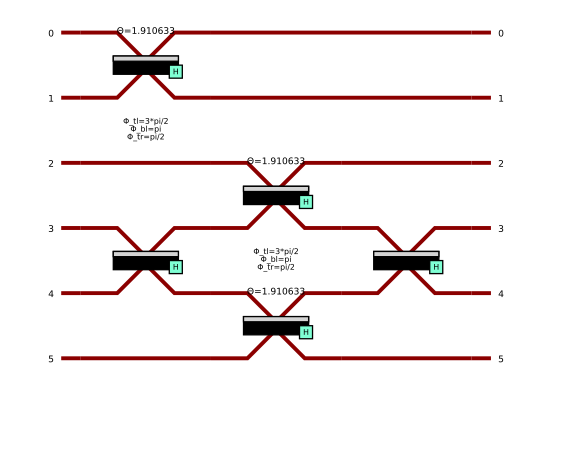
\includegraphics{parceval-example-cnot.png}
\caption{Wynik wykonania przykładowego kodu w pakiecie Parceval}
\end{figure}

\hypertarget{ux17aruxf3dux142a}{%
\paragraph{Źródła}\label{ux17aruxf3dux142a}}

\begin{enumerate}
\def\labelenumi{\arabic{enumi}.}
\tightlist
\item
  https://www.insidequantumtechnology.com/news-archive/pasqal-rolls-out-no-code-development-platform-pulser-studio/
\item
  Exploring the Features of Pulser Studio,
  https://www.pasqal.com/articles/pulser-s-1, 06/01/2023
\item
  Silvério, Henrique, Sebastián Grijalva, Constantin Dalyac, Lucas
  Leclerc, Peter J. Karalekas, Nathan Shammah, Mourad Beji, Louis-Paul
  Henry, and Loïc Henriet. ``Pulser: An open-source package for the
  design of pulse sequences in programmable neutral-atom arrays.''
  Quantum 6 (2022):
  629.https://quantum-journal.org/papers/q-2022-01-24-629/
\item
  https://pulserstudio.pasqal.cloud/
\item
  https://github.com/pasqal-io/Pulser
\item
  https://cloud.quandela.com/
\item
  Heurtel, Nicolas, Andreas Fyrillas, Grégoire de Gliniasty, Raphaël Le
  Bihan, Sébastien Malherbe, Marceau Pailhas, Eric Bertasi et
  al.~``Perceval: A software platform for discrete variable photonic
  quantum computing.'' Quantum 7 (2023): 931.
  https://quantum-journal.org/papers/q-2023-02-21-931/
\item
  https://perceval.quandela.net/
\end{enumerate}


\end{document}
